\section{Versuchsaufbau und Versuchdurchführung}

\subsection{Bestimmung der Zeitkonstante beim Entladevorgang}

\begin{flushleft}
    Die Schaltung wird wie in Abbildung \ref{Abbildung1} aufgebaut. 
    Durch einen Frequenzgenerator wird eine Rechtecksignal der Stärke $f = 200\,\unit{\hertz} $ generiert und läuft über ein Kabel durch den RC-Kreis und danach durch ein Kabel in das Oszilloskop.
    Auf dem Oszilloskop kann die Entladekurve dann betrachtet werden. Dies wird mit einem Foto festgehalten.
\end{flushleft}

\begin{figure}[H]     
    \centering
    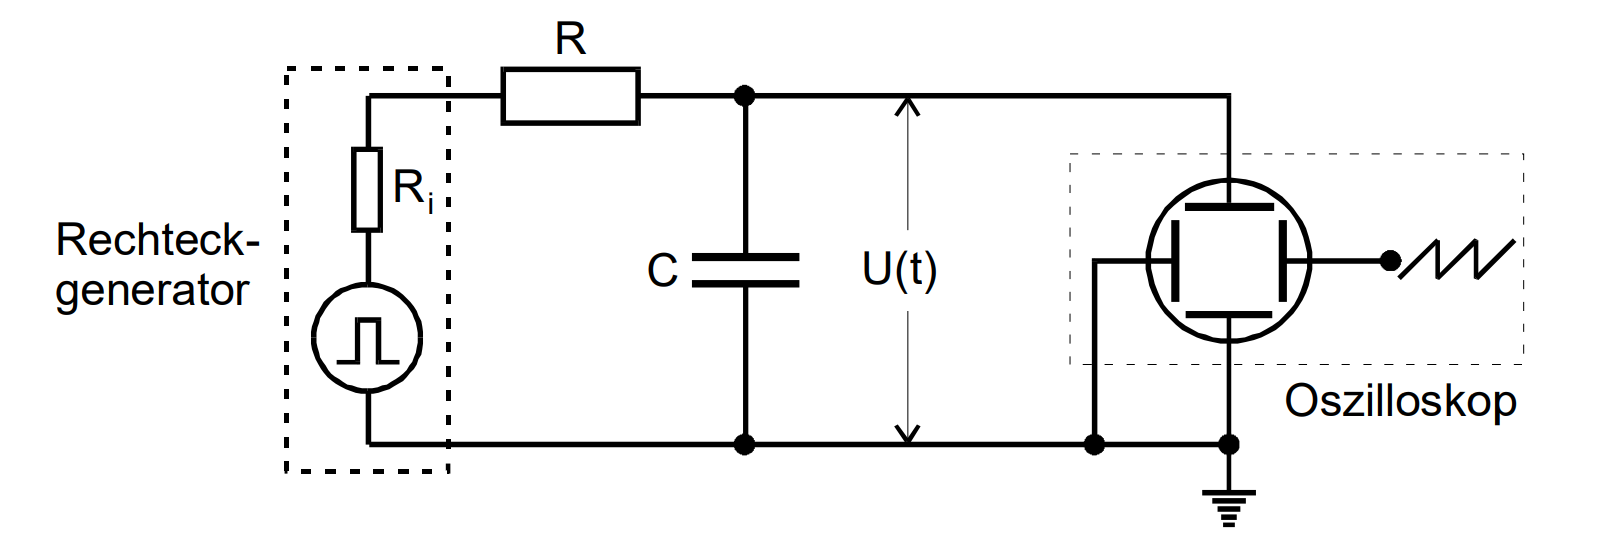
\includegraphics[width=140mm]{bilder/Abbildung1.png}
    \caption{Der Aufbau zur Bestimmung der Zeitkonstante \cite{a1}.\label{Abbildung2} }
\end{figure}

\subsection{Messung der Amplitude des Kondensators und der Phasenverschiebung}

\begin{flushleft}
    Der Schaltung von dem Durchgang davor wird ein Kabel ergänzt. 
    Dieses Kabel führt von dem Frequenzgenerator direkt zum Oszilloskop.
    Es werden Frequenzen von  $ 20\,\unit{\hertz} \leq f \leq 20000\,\unit{\hertz} $ eingestellt und die Amplitude von der Eingangsspannung $U_{\text{ein}}$, die Amplitude der Ausgangsspannung $U_{\text{aus}}$ , sowie die Phasenverschiebung $\varphi$ zwischen beiden Phasen.
\end{flushleft}

\begin{figure}[H]      
    \centering
    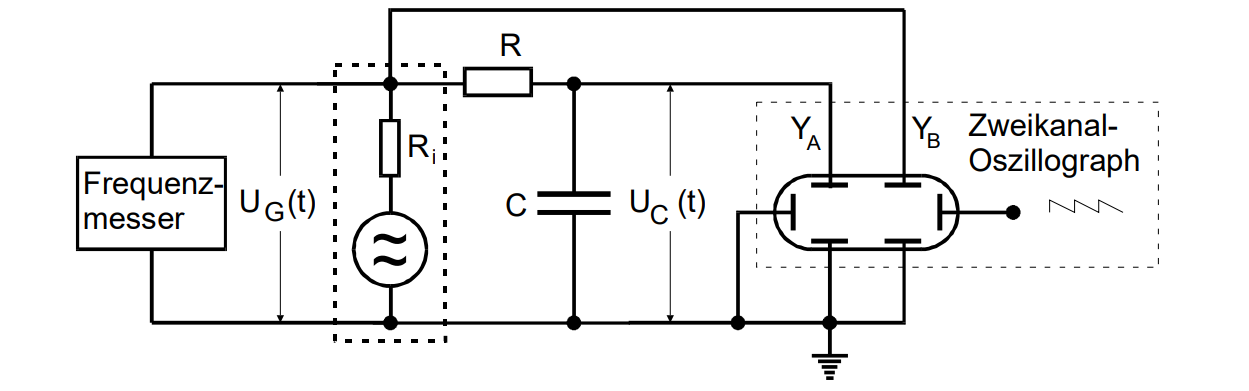
\includegraphics[width=140mm]{bilder/Abbildung3.png}
    \caption{Der Aufbau zur Messung der Amplitude und der Phasenverschiebung \cite{a1}.\label{Abbildung3} }
\end{figure}

\subsection{Bestätigung des RC-Kreises als Integrator}

\begin{flushleft}
    Der Aufbau des vorherigen Arbeitsauftrages wird beibehalten und der Verlauf der eingehenden sowie ausgehenden Spannungsverlauf mit einem Foto festgehalten.
    Durchgeführt wird dies einmal als Sinussignal, einmal als Dreieckssignal und einmal als Rechteckssignal. Die Frequenz wird auf $20\,\unit{\kilo\hertz}$.
\end{flushleft}
